%% LyX 1.5.1 created this file.  For more info, see http://www.lyx.org/.
%% Do not edit unless you really know what you are doing.
\documentclass[twocolumn,english]{article}
\usepackage[latin9]{inputenc}
\usepackage{geometry}
\geometry{verbose,a4paper,tmargin=28.3mm,bmargin=43.3mm,lmargin=80mm}
\setlength{\parskip}{\medskipamount}
\setlength{\parindent}{0pt}
\usepackage{graphicx}

\makeatletter
%%%%%%%%%%%%%%%%%%%%%%%%%%%%%% Textclass specific LaTeX commands.
\newenvironment{lyxcode}
{\begin{list}{}{
\setlength{\rightmargin}{\leftmargin}
\setlength{\listparindent}{0pt}% needed for AMS classes
\raggedright
\setlength{\itemsep}{0pt}
\setlength{\parsep}{0pt}
\normalfont\ttfamily}%
 \item[]}
{\end{list}}

%%%%%%%%%%%%%%%%%%%%%%%%%%%%%% User specified LaTeX commands.
\usepackage{latex8}
\usepackage{times}
%\documentclass[times,9pt,twocolumn]{article}


% \bibliographystyle{latex8}

\date{}

%\usepackage{type1cm}
%\renewcommand\normalsize{%
%   \@setfontsize\normalsize{9pt}{12pt}
%   \abovedisplayskip 10\p@ \@plus2\p@ %\@minus5\p@
%   \abovedisplayshortskip \z@ \@plus3\p@
%   \belowdisplayshortskip 6\p@ \@plus3\p@ %\@minus3\p@
%   \belowdisplayskip \abovedisplayskip
%   \let\@listi\@listI}
%\normalsize  

\sloppy

  \let\oldthebibliography=\thebibliography
 \let\endoldthebibliography=\endthebibliography
  \renewenvironment{thebibliography}[1]{%
    \begin{oldthebibliography}{#1}%
      \setlength{\parskip}{0ex}%
      \setlength{\itemsep}{0ex}%
  }%
  {%
    \end{oldthebibliography}%
  }

\usepackage{babel}
\makeatother

\begin{document}

\title{Extensible Systems: Plugin versus Component Substitution Architectures}


\author{Andrew McVeigh, Jeff Kramer and Jeff Magee\vspace{4pt}\\
Department of Computing\\
Imperial College\\
London SW7 2BZ, United Kingdom\\
\{amcveigh, jk, jnm\}@doc.ic.ac.uk}

\maketitle
\begin{abstract}
\textit{Many extensible systems are delivered in the form of a base
application with a plugin architecture. Plugins can be added to the
application to extend its functionality, allowing it to be tailored
for different needs.}

\textit{We introduce component substitution architectures as an alternative
to this style, providing a more flexible and granular extension model.
This approach is also shown to cope well with unplanned extension.
We demonstrate how substitution, combined with a structural form of
component inheritance called resemblance, can be used to effectively
model and extend a system.}

\textit{To evaluate both styles, we examine part of the architecture
of the Eclipse development tool and indicate how each approach would
handle the same extension requirement. Component substitution is shown
to more naturally model the situation, with the further advantage
that the cost of introducing the extension is closely aligned to the
size of the change required to the architecture.}
\end{abstract}

\section{Introduction}

One way to structure an extensible system is to provide a base application
with predefined extension points where the application can be extended.
Developers create plugins, which {}``plug into'' the extension points,
and these plugins can then be selectively added to an installation
of the application to customize it \cite{Volter1999}. The base application
acts as a platform, providing a substrate for a family of applications.

This approach is referred to as a plugin architecture and the basic
concepts can be succinctly described using a simple design pattern
\cite{Volter1999,Mayer2003}. Advanced plugin architectures, such
as Eclipse \cite{Object2001}, allows plugins to also offer extension
points which can then be further extended by other plugins. The model
in \cite{Chatley2003} also supports this feature, but calls extension
points {}``holes'' and the elements that extend them {}``pegs''.

One of the benefits of the plugin architectural style is that plugins
can be created by developers who are not affiliated with the original
application developers. The original developers are then fee to concentrate
on the base platform without having to continually expand the system
to cater for every requirement.

Examples of successful applications using this approach are the Eclipse
Integrated Development Environment \cite{Object2001a} and Firefox
\cite{Firefoxplugins2008}. The COM add-in model of the Microsoft
Office suite \cite{Microsoft2006,Microsoft2006a} could also be regarded
as another example of this style.

The plugin model primarily facilitates additive change to a system,
according to the extension points defined already in the base. Extending
and customizing a system can involve more than just addition, however.
We use the term \emph{extension} to refer to a unit (analogous to
a plugin) that can add, replace or delete functionality {[}ref]. The
plugin concept is a therefore a subset of the extension concept.

The component substitution model is offered as an alternative to the
plugin approach. The foundation of this approach is to allow an extension
to substitute any other application component with one of its own.
Combined with resemblance, which allows components to structurally
inherit from each other, an extension can incrementally modify any
part of a system providing great flexibility to reshape the architecture
to meet new requirements.

Backbone is an architecture description language (ADL) developed as
part of this work to demonstrate the component substitution concepts.
The Backbone model also builds on ADLs such as Darwin \cite{Kramer2000}
and UML2 \cite{Selic2003}, which provide full hierarchical component
models. It therefore features a robust and practical component model
at its core, as well as offering extension constructs which augments
this. The aim is to make extension as natural an engineering process
as initial creation, and to cope with unplanned change by allowing
any part of a system to effectively become an extension point. This
lifts the burden off developers to factor in predictive extension
points.

To evaluate the two approaches, we consider a modification to the
Eclipse integrated development environment. This is modeled with the
Eclipse plugin approach, and also in Backbone allowing direct comparison
of the two styles.

The rest of the paper is structured as follows. Section \ref{sec:Extending-a-Plug-In}
examines the characteristics of plugin architectures, focusing specifically
on the Eclipse model. Section \ref{sec:Backbone-and-Component} introduces
the component substitution approach and the Backbone ADL)which embodies
these concepts. Section \ref{sec:A-Formal-Model} presents the outline
of a formal model for Backbone, showing various properties that result.
Related work is reviewed in section \ref{sec:Related-Work} and section
\ref{sec:Conclusions-and-Future} presents conclusions and discusses
further work.


\section{\label{sec:Extending-a-Plug-In}Extending a Plug-In Architecture}


\subsection{Anatomy of a Plug-In Architecture}

A basic plugin design pattern is described in \cite{Mayer2003}. Figure
\ref{fig:A-UML-class} expands on this to present a UML class diagram
of a more general model, which describes the Eclipse approach where
plugins can also be extended. The distinction between plugins and
the base application is therefore blurred, as the base is a relative
concept which can be thought of as a system loader and a given collection
of plugins. This is certainly the case in Eclipse, where even the
fundamental run-time and editing concepts reside in plugins.

%
\begin{figure}[h]
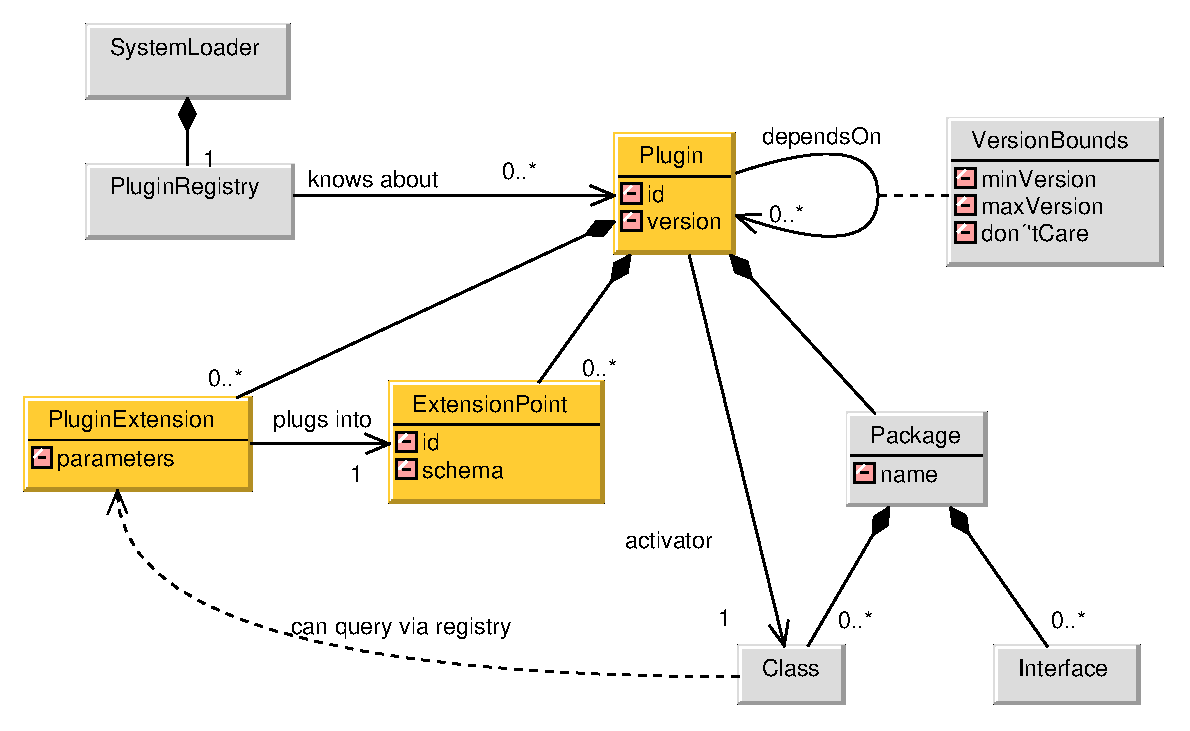
\includegraphics[width=1\columnwidth]{images/plug-in-model}

\caption{\label{fig:A-UML-class}The plugin model}

\end{figure}


SystemLoader is the class which bootstraps the initial system, discovers
any Plugins and registers them with the PluginRegistry. The registry
knows about all Plugins, and can be used to query for a specific Plugins
via the {}``id'' and {}``version'' attributes.

A Plugin is a versioned collection of packages, classes and interfaces.
A Plugin may depend on other Plugins, and the VersionBundle association
class shows that this dependency can be expressed as a reference to
a specific Plugin version, a bounded set of versions, or no particular
version ({}``don'tCare'').

A Plugin may provide a set of PluginExtensions which connect into
the ExtensionPoints of other Plugins. A PluginExtension uniquely identifies
the relevant ExtensionPoint by its identifier ({}``id''). A Plugin
may further define its own set of ExtensionPoints, each of which declares
which parameters must be supplied (conforming to {}``schema'') by
a PluginExtension of one or more other Plugins. Note that this model
allows an ExtensionPoint to accept multiple PluginExtensions, although
any given PluginExtension can only plug into one ExtensionPoint. The
motivation is that if an ExtensionPoint allowed only a single PluginExtension,
then multiple Plugins could all try to fill the point, and conflict.

(In Eclipse, the actual terminology for a PluginExtension is {}``extension''.
We have used PluginExtension to differentiate this concept from our
notion of an extension as being analogous to a plugin that can add,
remove and replace functionality)

At run-time, the set of Plugins are discovered and registered, and
the PluginExtensions matched up to ExtensionPoints. Control is then
passed to a particular Plugin, often one plugged into a distinguished
ExtensionPoint designed for bootstrapping. Each Plugin is able to
query the PluginExtensions which extend its points, and the parameters
passed can include class names (for object instantiation) and values.

The extensibility of the approach comes from Plugins not knowing (or
needing to know) what PluginExtensions will be provided for their
extension points until run-time. The actual PluginExtensions for a
Plugin's extension points is a function of how many extending Plugins
are discovered in the environment.

An ExtensionPoint is equivalent to a number of optionally required
interfaces (to handle the multiplicity), and a PluginExtension is
equivalent to a provided interface. Rather than model these concepts
directly using interfaces, however, the Eclipse model expresses the
data required and provided via meta-data (XML files). Some of this
data can refer directly to class names, and a Plugin can choose to
instantiate an object based on a class name passed to its extension
point.


\subsection{\label{sub:Extending-Eclipse:-Adding}Extending Eclipse: Adding a
Column to the Task View}

As a case study, we chose to enhance a small aspect of the Eclipse
(version 3.3) task view. As shown in figure \ref{fig:The-task-view},
this shows a list of tasks along with certain columns. We wish to\emph{
add} a further column {}``assigned to'' in order to show which person
has been allocated the task.

%
\begin{figure}[h]
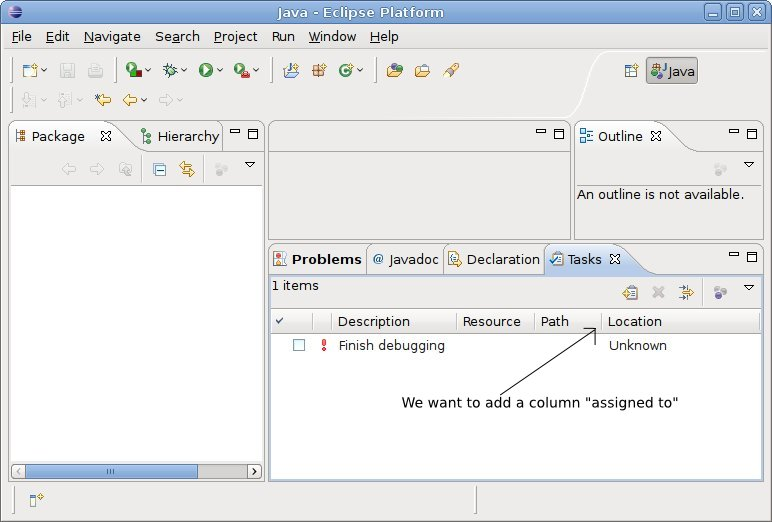
\includegraphics[width=1\columnwidth]{original-images/tasks}

\caption{\label{fig:The-task-view}The Eclipse task view}

\end{figure}


The first step in making the addition is to find the plugin responsible
for viewing tasks. This proved to be straight forward: a class called
TaskView exists in the\emph{ org.eclipse.ui.ide} plugin. However,
there is a problem. Looking at the source code for this class shows
the set of columns to be hard-coded in the TaskView class itself.

\begin{lyxcode}
{\scriptsize public~class~TaskView~extends~MarkerView~\{}{\scriptsize \par}

{\scriptsize{}~~~~...}{\scriptsize \par}

{\scriptsize{}~~~~private~final~IField{[}]~VISIBLE\_FIELDS~=}{\scriptsize \par}

{\scriptsize{}~~~~~~~\{~new~FieldDone(),~new~FieldPriority(),}{\scriptsize \par}

{\scriptsize{}~~~~~~~~~new~FieldMessage(),~new~FieldResource(),}{\scriptsize \par}

{\scriptsize{}~~~~~~~~~new~FieldFolder(),~new~FieldLineNumber()~\};}{\scriptsize \par}

{\scriptsize{}~~~~...}{\scriptsize \par}
\end{lyxcode}
The developers clearly did not anticipate extension in this way. We
must look for an alternative approach.

In an ideal world, it would be possible to simply create a new plugin,
with a new EnhancedTaskView class and substitute this class for the
existing TaskView class. This is the intent of the substitution facilities
in component substitution architectures. However, since the plugin
model primarily facilitates addition, this type of effect is not possible.

Examining the meta-data (plugin.xml file) for this plugin shows how
the task view is instantiated. The PluginExtension declaration references
the TaskView class and plugs into the appropriate extension point,
as shown below. (Note that the following is a declaration of an extension,
rather than an extension point, which has a tag of extension-point)

\begin{lyxcode}
{\scriptsize <extension~point=\char`\"{}org.eclipse.ui.preferencePages\char`\"{}>}{\scriptsize \par}

{\scriptsize{}~~<view~name=\char`\"{}\%Views.Task\char`\"{}}{\scriptsize \par}

{\scriptsize{}~~~~icon=\char`\"{}\$nl\$/icons/full/eview16/tasks\_tsk.gif\char`\"{}}{\scriptsize \par}

{\scriptsize{}~~~~category=\char`\"{}org.eclipse.ui\char`\"{}}{\scriptsize \par}

{\scriptsize{}~~~~class=}{\scriptsize \par}

{\scriptsize{}~~~~~\char`\"{}org.eclipse.ui.views.markers.internal.TaskView\char`\"{}}{\scriptsize \par}

{\scriptsize{}~~~~id=\char`\"{}org.eclipse.ui.views.TaskList\char`\"{}>}{\scriptsize \par}

{\scriptsize{}~~</view>}{\scriptsize \par}

{\scriptsize </extension>}{\scriptsize \par}
\end{lyxcode}
If we could change this file we could substitute our EnhancedTaskView
class as the parameter and our new view would be used instead of the
previous one. However, the plugin.xml file lives in the org.eclipse.ui.ide
plugin itself, and to replace the lines, we must create a new version
of the plugin.

Creating a new version is not a perfect solution, however, due to
other characteristics of the model. Firstly, the plugin consists of
around 300 Java classes, and we must edit the source and introduce
a new version of the plugin. The effort required in forking this plugin
is vastly out of proportional to the small architectural addition
required.

Furthermore, introducing a new version will cause a problem if any
plugins explicitly declare a dependency on the old version. We will
end up in that case with two referenced versions of the plugin (old
and new), and concurrent versions of the same plugin are not allowed
in Eclipse for anything that contributes to extension points \cite{Birsan2005}.
Even if this were allowed, having two concurrent versions of a plugin
holding shared state would not be a desirable outcome.

As such, Eclipse plugins follow a convention. All dependencies on
plugins are expressed as a version range from 3.0.0 up to (but not
including) 4.0.0. The leftmost digit of the versioning scheme indicates
breaking API changes. Without this approach, we would not be able
to easily introduce even a minor, non-breaking change. It is not possible
to introduce a breaking change without also creating a new version
of all plugins (incrementing the leftmost digit) which depend on this
plugin, and so on in cascade fashion. This certainly constrains the
type of change we can introduce, even if we are willing to update
any upstream artifacts which have issues with the change. We will
end up having to update most of the plugins in the system.

Even creating a new non-breaking version has its issues and is likely
to be a short term solution. It is known that Eclipse 3.4 is introducing
a new version of this plugin, with an enhanced task view that colors
tasks according to priority. As it is not possible to run two versions
concurrently, we will have to accept the fact that we must merge our
source changes into each new release of the plugin. Regardless of
how important we view our change, it is unlikely that the maintainer
(the Eclipse Foundation) will incorporate our (and everyone else's)
changes into the plugin that they own and maintain.


\subsection{Coarse Grained Plugins}

A key problem in the above scenario is the coarseness of plugins.
If the plugins could somehow be made more fine-grained with extension
points for every conceivable scenario then the problem would be simpler
to solve.

A tension exists, however, between making the architecture fine-grained
and making it manageable and understandable. If we make plugins too
small, we will end up with literally many thousands. As shown by figure
\ref{fig:Part-of-the}, the plugin structure for Eclipse is already
complex. The figure shows around 80 plugins, a typical environment
contains around 200, and an enterprise product based on Eclipse is
known to contain over 500. Having more plugins implies a less manageable
system. Some form of nesting or composition would address this, at
least providing a way to view the system at multiple levels.

%
\begin{figure}
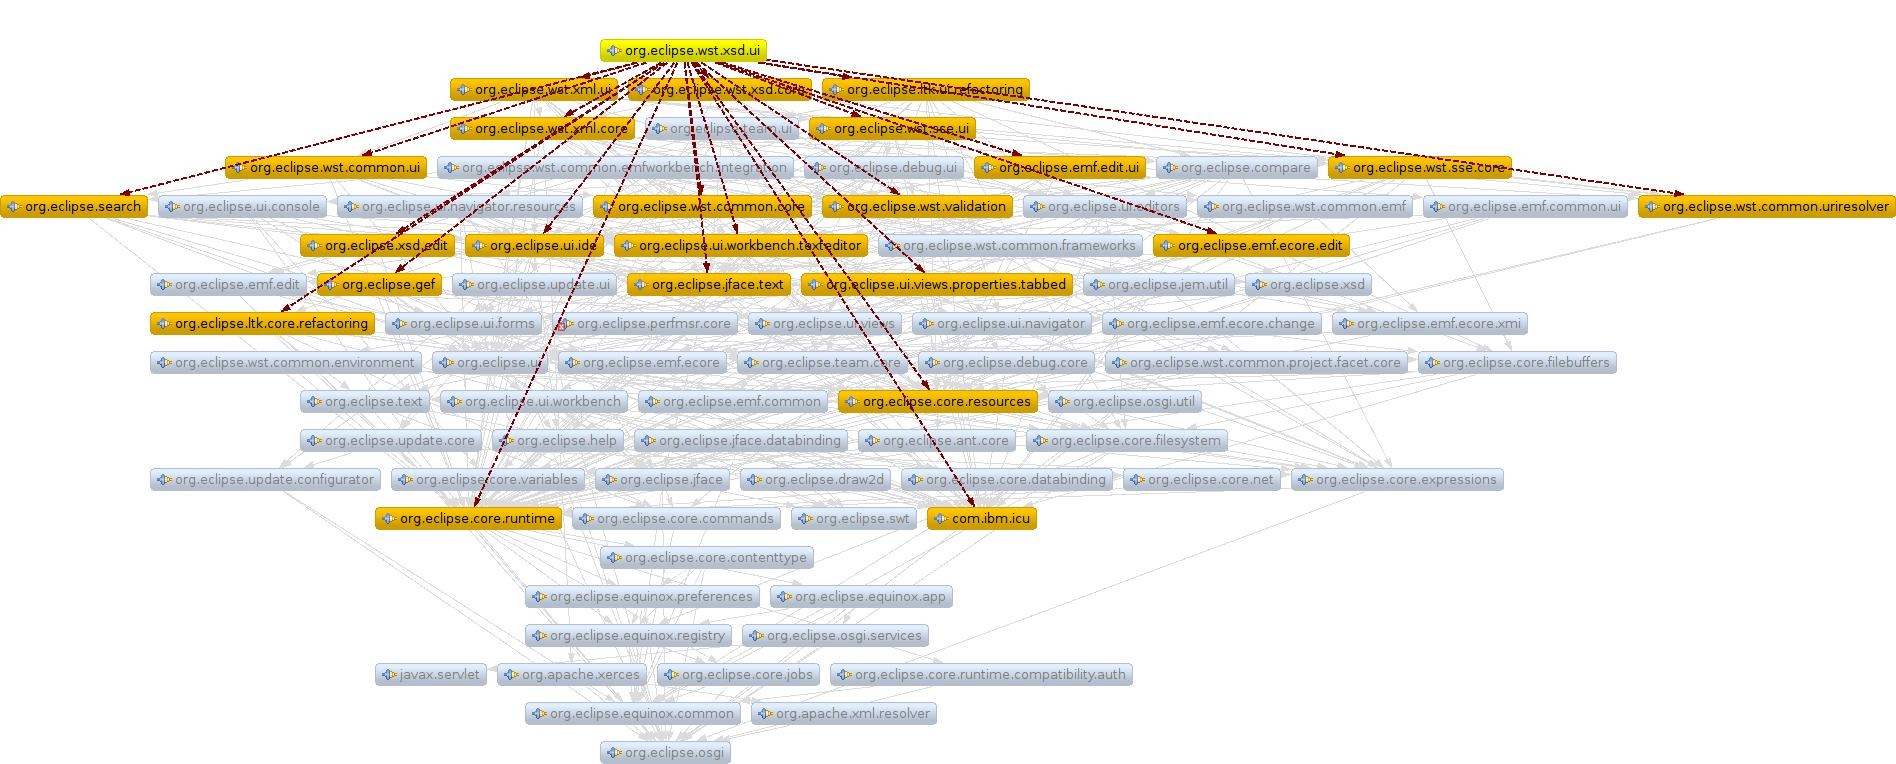
\includegraphics[width=1\columnwidth]{original-images/tangle}

\caption{\label{fig:Part-of-the}Part of the Eclipse plugin dependency graph}

\end{figure}


(Note that Eclipse plugins have names conforming to Java-like conventions.
However, like Java packages, the name is just a convention and does
not indicate any precise nesting. Attempts to simulate the effect
of composition by using the names reduced little of the complexity
and gave an incorrect view of the architecture)


\subsection{\label{sub:Characteristics-of-the}Characteristics of the Eclipse
Plug-In Model}

Eclipse plugins are closely related to the concept of subsystem {[}ref].
Like a subsystem, and unlike Backbone components, a plugin can only
be instantiated once. A subsystem requires certain interfaces (ExtensionPoints)
and provides others (PluginExtensions).

The plugin model is essentially additive. Any extension beyond addition
requires that a new version of an existing plugin be created. As shown,
even minor changes can lead to this situation.

Our small example require a new version of a plugin. This presented
several problems. Firstly, the plugin is a sizable artifact due to
the lack of composition, and creating a new version is a change that
is out of proportion to the size of the architectural change (addition)
required. Next, introducing a new version can lead to a situation
where multiple concurrent versions of a plugin are implied, which
is prohibited according to the rules of the platform. Finally, creating
a new version leads to its own problems in that we are not the main
developers of this plugin and will therefore have to acquiesce to
performing a source level merge of our changes whenever a new version
is published by the Eclipse Foundation.

As it turns out, our small change was not planned for -- the creators
of the plugin did not anticipate or cater for this type of change
via addition. This is an interesting characteristic in that unplanned
changes, even those notionally adding a feature, must be characterized
as replacement. If the requirement had been foreseen, an extension
point could have been provided to allow the registration of extra
columns for the task view in an additive fashion. Clearly, however,
anticipating all future changes is a costly and largely unrewarding
exercise. The architecture will become unnecessarily polluted with
extension points, creating a lot of development work which in turn
may not in fact capture all possible future requirements.

The issues found in this example relate closely to the requirements
presented in our work on component reuse \cite{McVeigh2006}. In that
paper we elaborated a set of requirements for effective component
reuse and extension. As Eclipse structures itself as a set of components,
we can assess its approach against these requirements. In this case,
the system fails to provide sufficient flexibility because we are
unable to make changes without copying and modifying the source code
for the plugin (ALTER, NOSOURCE). We are also unable to seamlessly
accept a new version without having to perform a source level merge
(UPGRADE). The requirement that changes have no impact (NO IMPACT)
on existing consumers of the plugin is met, as there is no need to
force the upgrade on those who do not wish to see the new version.

As it is, the Eclipse plugin model contains practical and undesirable
limitations on how easily a system can be extended, understood and
managed. The next section introduced component substitution architectures,
which provide constructs which remove or ameliorate the limitations
so far discussed.


\section{\label{sec:Backbone-and-Component}Component Substitution Architectures}


\subsection{Concepts}

The foundation of the substitution approach is an extension, which
is a packaged collection of interfaces and components. An extension
is loosely analogous to a plugin.

Unlike a plugin, however, an extension can choose to substitute any
component (in the system being extended) with one of its own. This
gives an extension the ability to re-make the underlying architecture
in order to effect any required changes. A further construct, called
resemblance, allows a component to inherit and incrementally modify
(add, delete, replace) the structure of other components. Together,
substitution and resemblance allow an extension to make an incremental
modification to an existing component in a system. This is termed
incremental substitution.

In the Eclipse example, a new extension could simply incrementally
substitute TaskView to add the new column. Although this approach
would work even when using a class-based model {[}mixjuice], there
are limitations related to inheritance. Classes primarily allow additive
extension (and a level of method replacement) through inheritance
which limits the type of extension. This was the motivation to introduce
a full component model, along with the resemblance construct which
allows incremental add, delete or replace of inherited structure.
The relationship between components and classes will be described
in this section.

An important element of the substitution approach is therefore a compositional
component model, where composite components are made up of instances
of other components. This allows an entire system to be structured
as a component which decomposes into other components and so on until
we reach fine-grained leaf components. This gives the ability to finely
decompose a system, letting any substitution to take place at the
appropriate level of abstraction. This allows the practical cost of
a change to be closely matched to the actual architectural change,
as will be shown as we apply these ideas to the Eclipse task view
example in the next section. Furthermore, because of the composition
hierarchy, the system is still manageable and understandable by viewing
the system at the require level of abstraction.

These concepts address the major issues found in the plugin example.
The model can be finely structured without becoming difficult to manage,
and incremental substitution makes any constituent of an existing
component into a potential extension point. Furthermore, component-based
resemblance provides a more powerful change model than class-based
inheritance, allowing more than just additive change.


\subsection{Modeling the Task View in Backbone}

This section explains the Backbone ADL through the task view extension
example.

The Backbone language has been developed as part of this work, in
order to evaluate the substitution model. Backbone features the substitution
and resemblance constructs, and a compositional component model where
each leaf component (components which are not further decomposable)
describes a Java class. As such, Backbone is able to provide an interpreter
which can assemble the system from an architectural description and
Java classes. Detailed motivation behind the constructs is described
in \cite{McVeigh2006}, although that paper refers to substitution
as {}``redefinition''.

Going back to the task view example of \ref{sub:Extending-Eclipse:-Adding},
consider modeling the concept of a view column (e.g. {}``description'')
in Backbone. Figure \ref{fig:A-component-definition} shows GridColumn
as a leaf component, which cannot be further decomposed. It has a
single attribute {}``name'' and provides an interface IGridColumn.
We will later use instances of this component to configure the task
view's visible columns.

%
\begin{figure}[h]
\noindent \begin{centering}
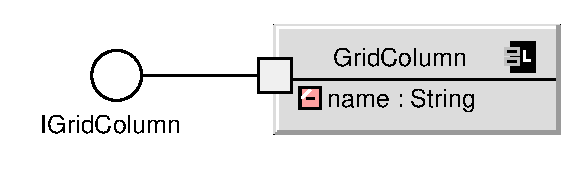
\includegraphics[width=0.4\columnwidth]{images/column}
\par\end{centering}

\caption{\label{fig:A-component-definition}A column component}



\end{figure}


As this is a leaf (note the {}``L'' in the top right corner), it
also describes a Java class. This is shown below. The component definition
is represented graphically (or textually) in Backbone and the implementation
is represented in Java.

\begin{lyxcode}
{\scriptsize public~class~GridColumn~\{}{\scriptsize \par}

{\scriptsize{}~~private~IGridColumn}{\scriptsize \par}

{\scriptsize{}~~~~g\_IGridColumnProvided~=}{\scriptsize \par}

{\scriptsize{}~~~~~~~~new~IGridProvidedImpl();}{\scriptsize \par}

{\scriptsize{}~~private~String~name;}{\scriptsize \par}

{\scriptsize{}~~}{\scriptsize \par}

{\scriptsize{}~~private~class~IGridProvidedImpl}{\scriptsize \par}

{\scriptsize{}~~~~~~~~implements~IGridColumn~\{}{\scriptsize \par}

{\scriptsize{}~~~~...}{\scriptsize \par}

{\scriptsize{}~~\}\}}{\scriptsize \par}
\end{lyxcode}
The grid user interface widget (figure \ref{fig:A-grid-widget}) displays
a set of columns and their associated data on the screen. It is the
user interface widget for displaying a task view, providing IGrid,
and requiring IGridColumn. The small box named {}``r'' indicates
a port, which allows a multiplicity to be added for interfaces provided
or required. The {[}0..{*}] therefore indicates that zero to many
provisions are required, thus giving the same effect as an extension
point which can accommodate many PluginExtensions.

%
\begin{figure}[h]
\noindent \begin{centering}
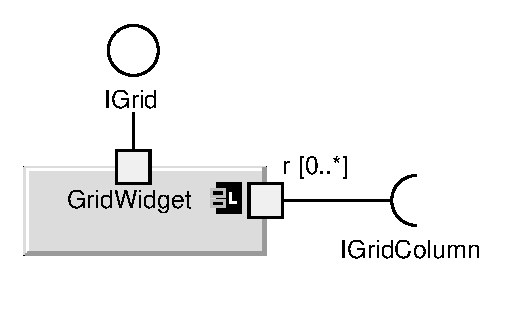
\includegraphics[width=0.4\columnwidth]{images/widget}
\par\end{centering}

\caption{\label{fig:A-grid-widget}A grid widget component}

\end{figure}


Required interfaces are analogous to extension points in Eclipse.
Provided interfaces are analogous to PluginExtensions, which provide
data to extension points. Interfaces are more flexible however, as
object references can be passed, in addition to data and class references.

A composite component is constructed out of instances of other components.
These instances, in the terminology of UML2, are known as parts \cite{OMGUML}.
A composite is effectively shorthand for instructions to wire up a
set of other parts. As such, all components can be {}``flattened''
into a connected set of leaf component instances {[}ref to raedstock].

Figure \ref{fig:The-task-viewer} shows the task view as a composite
component. The inner boxes are instances of other components (parts).
In this case, there are two columns ({}``Description'', {}``Location'')
configured up to the grid widget part. Note also that TaskView resembles
MarkerView (fully shown). The instances of MarkerViewController and
GridWidget are structurally inherited from MarkerView, which defines
a generic type of view of marker information. TaskView has added the
two GridColumn parts.

Note that TaskView is not a leaf, and therefore does not have a Java
representation. Instances of this component must be constructed from
Backbone, which will flatten the component hierarchy and connect together
leaf object instances.

%
\begin{figure}[h]
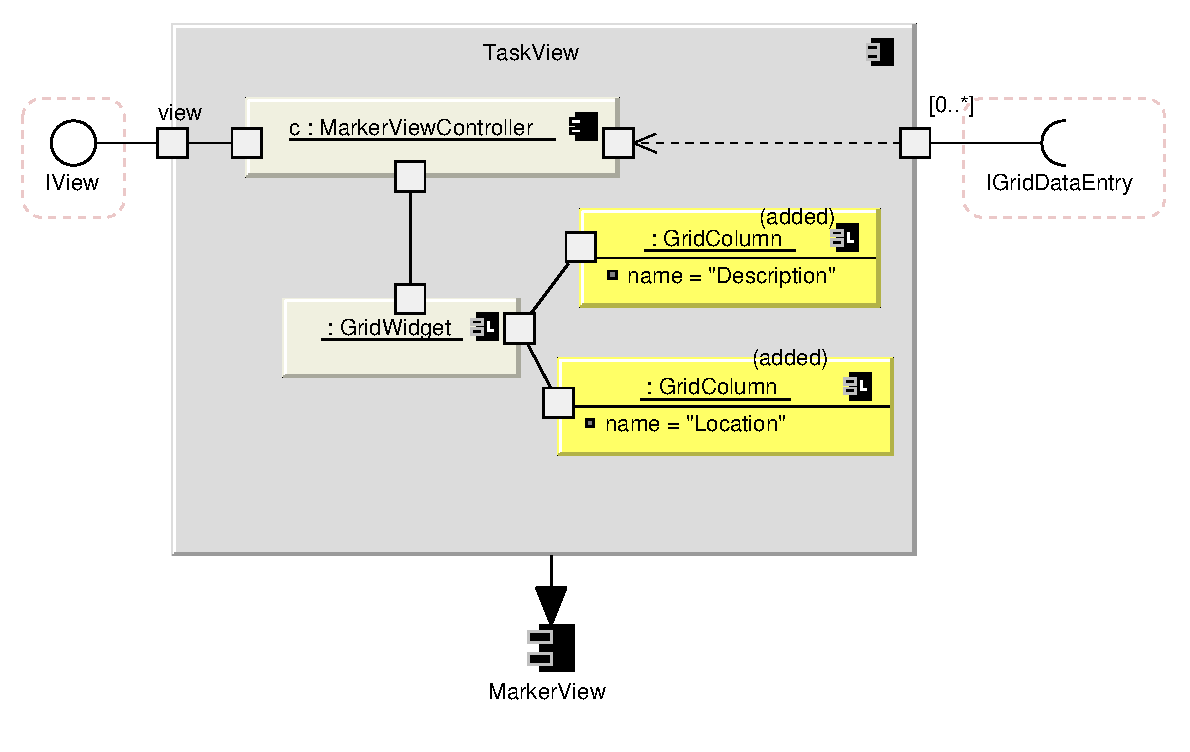
\includegraphics[width=1\columnwidth]{images/taskviewer}

\caption{\label{fig:The-task-viewer}The task view component}



\end{figure}


Finally, all the components and interfaces are bundled up into a module-like
construct known as a stratum (figure \ref{fig:The-taskview-and})
A stratum constitutes a unit of extension that can be applied to an
application, loosely analogous to a plugin. The taskview stratum packages
up TaskView, and the entire unit is dependent upon (and can legally
refer to) the definitions in the markerview stratum. 

%
\begin{figure}[h]
\noindent \begin{centering}
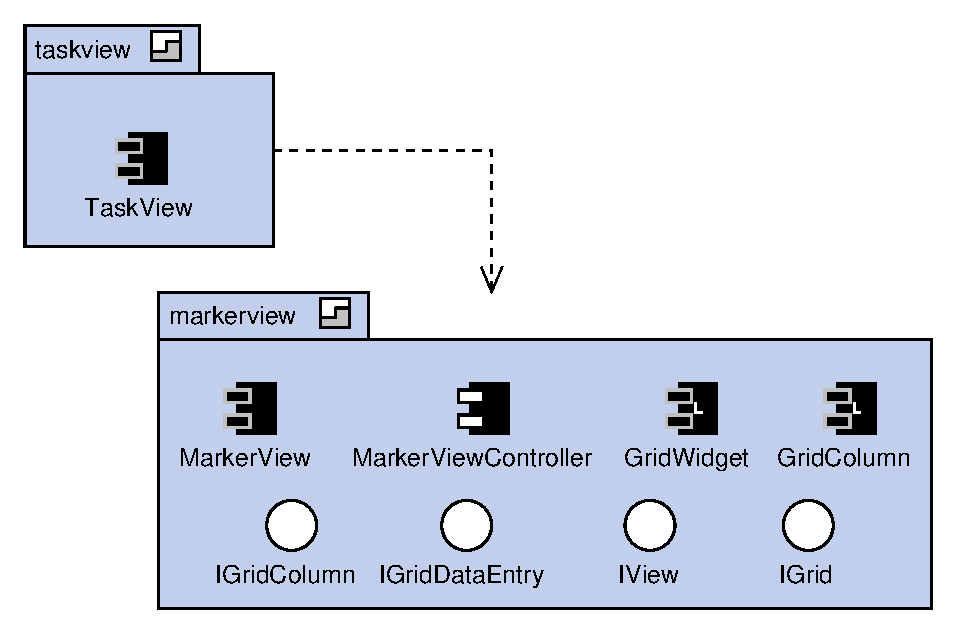
\includegraphics[width=0.8\columnwidth]{images/base-stratum}
\par\end{centering}

\caption{\label{fig:The-taskview-and}The taskview and markerview strata}



\end{figure}


Technically, a stratum is a stereotyped UML2 package. It uses different
rules for package visibility, nesting and export to be more compatible
with extensible systems. They aim to avoid the modularity limitations
on the package construct, summarized in {[}ref to UML module paper].
The strata rules are not further explained in this paper. 


\subsection{Extension via Substitution}

The TaskView and associated elements model the existing Eclipse task
view, before our requirement to add the {}``assigned to'' column.
Our extension will need to add the extra column, and to give an example
of replacement, we are supposing that the MarkerViewController instance
also needs to be enhanced to display the new column. To achieve this
effect, we create a further stratum, called enhancedtaskview, which
contains an incremental substitution of TaskView. The substitution,
shown as TaskView` is shown in figure \ref{fig:The-component-that}.
The dual headed arrow between TaskView` and TaskView denotes incremental
substitution (resemblance and substation together).

%
\begin{figure}
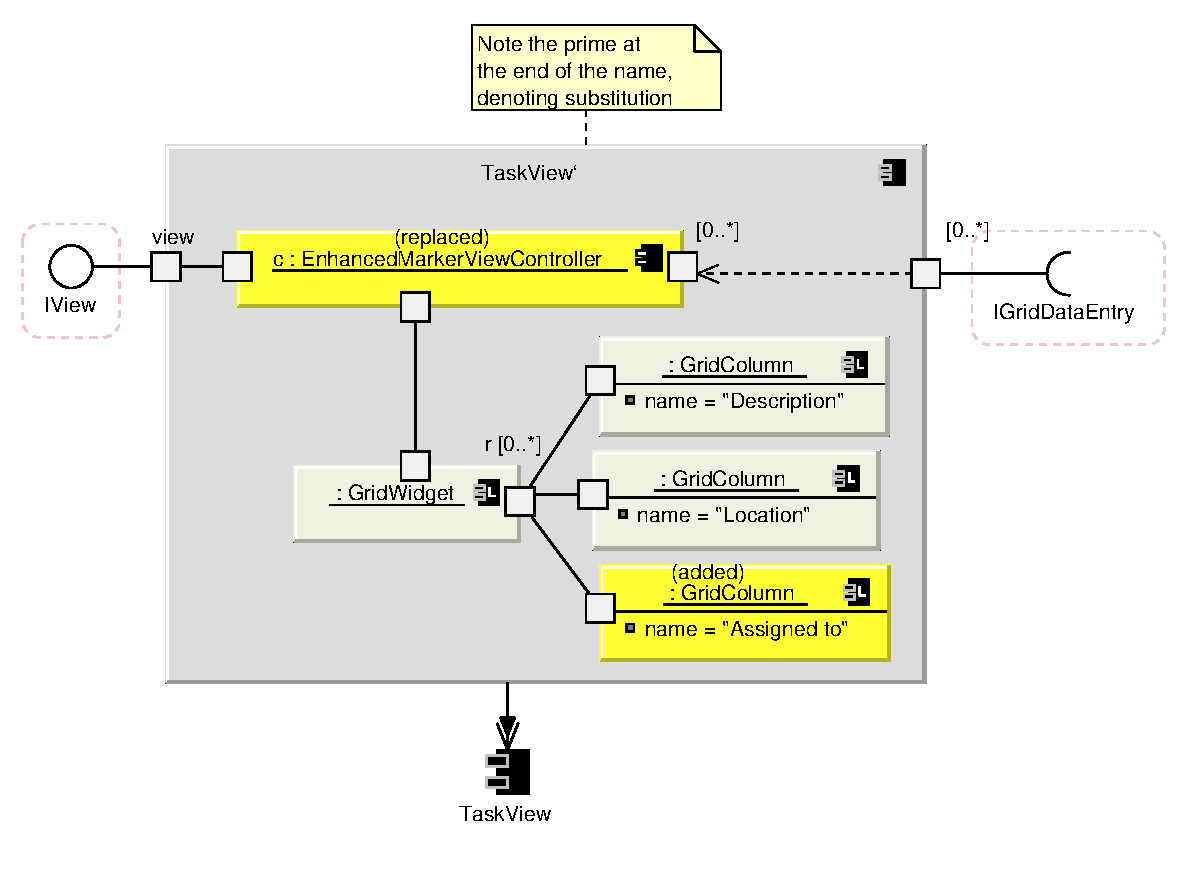
\includegraphics[width=1\columnwidth]{images/enhanced-taskview}

\caption{\label{fig:The-component-that}An incrementally substitution of TaskView}



\end{figure}


The TaskView` component has replaced the MarkerViewController part
with an instance of EnhancedMarkerViewController and added a GridColumn
part for our new column. All other parts are inherited from the original
TaskView.

The component is packaged into a stratum as shown in figure \ref{fig:Packaging-up-the}.
We can create a system that includes this stratum, thereby applying
the substitution and getting the additional column, or we can exclude
it and recreate the original task view.

%
\begin{figure}[h]
\noindent \begin{centering}
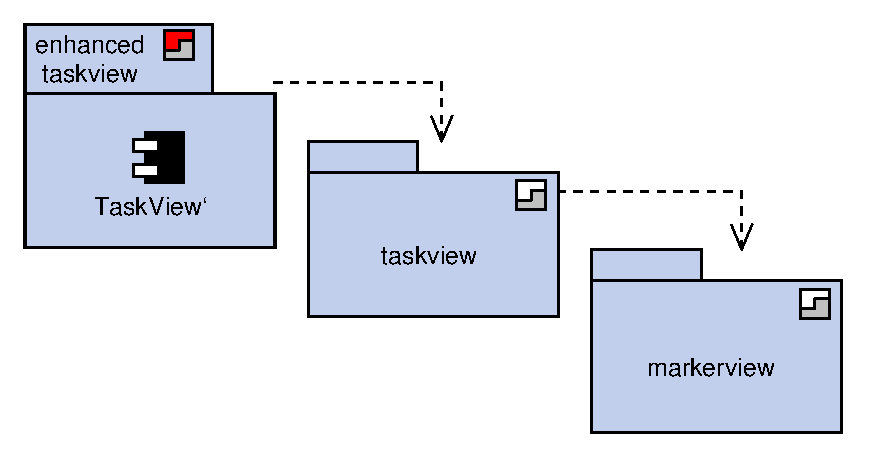
\includegraphics[width=1\columnwidth]{images/extension}
\par\end{centering}

\caption{\label{fig:Packaging-up-the}Packaging up the extension}



\end{figure}



\subsection{Resemblance as Deltas}

It is vital to note that any resembling component is held as a set
of deltas. For instance, the textual Backbone description of the substituting
component (omitting the extra connector) is as follows:

\begin{lyxcode}
{\scriptsize \{}~\\
{\scriptsize{}~component-name:~TaskView`}~\\
{\scriptsize{}~substitutes:~taskview::TaskView}~\\
{\scriptsize{}~resembles:~taskview::TaskView}~\\
{\scriptsize{}~parts:~\{~type:~taskview::GridColumn,}~\\
{\scriptsize{}~~slots:~\{~attributes:}~\\
{\scriptsize{}~~~~~\{~name:~name,~type:~String,}~\\
{\scriptsize{}~~~~~~~value:~\char`\"{}Assigned~to\char`\"{}~\}\}\}}{\scriptsize \par}

{\scriptsize{}~replaceParts:~\{}~\\
{\scriptsize{}~~original:~taskview::TaskView.c,}~\\
{\scriptsize{}~~part:\{}{\scriptsize \par}

{\scriptsize{}~~~type:~enhancedtaskview::EnhancedMarkerViewController\}\}}~\\
{\scriptsize \}}{\scriptsize \par}
\end{lyxcode}
The substituting component has replaced the part {}``c'' with an
EnhancedMarkerViewController part and added a GridColumn part. All
other parts (figure This \ref{fig:The-component-that}) are inherited
from the original TaskView definition. Resemblance allows for part,
port, attribute and connector addition, replacement and deletion.

The use of deltas is important, as it allows the base component to
be changed at a later point without introducing copying errors. A
change to the base may happen through simple editing, or a further
substitution when an upgrade occurs or another extension is applied.

In this approach, an evolution of a system can also be packaged as
an extension. The deltas in this substitution above and the deltas
from the evolution can both be applied, satisfying the UPGRADE requirement
outlined in \ref{sub:Characteristics-of-the}. This gives us the freedom
to make modifications to components of which we are not the primary
maintainer, which is difficult in the plugin model. The model will
simply combine our changes with those of the upgrade, using strata
dependencies to order the application of the deltas. In cases where
only a partial strata order is present (e.g. diamond-shaped dependencies)
then multiple resemblance is used (see \ref{sec:A-Formal-Model}).


\subsection{Characteristics of the Component Substitution Model}

The component model used is hierarchical, allowing components to be
decomposed to a fine-grained level. This in turn allows any substitution
to be more targeted than in the plugin model. Changes can be made
at the appropriate level of abstraction.

Further, any element of the model (component, part, attribute, connector
etc) is a natural extension point, as it can be replaced via a substitution.
Unlike the plugin model which requires advance planning for extension,
the ability to extend is a seamless part of creating a system in the
substitution model and extension points become more fine grained as
the model is elaborated.

Using a component model rather than a class model allows the internal
structure of each artifact to be displayed graphically. As all component
creation is controlled via Backbone, and is present in the graphical
model as parts, the architecture is more understandable than a class-based
model that hides object instantiation implicitly in code. Furthermore,
resemblance is more powerful than inheritance, allowing deletion and
replacement as well as addition. The tie between the Backbone model
and the Java implementation is expressed at the leaf component level.

Resemblance keeps any changes, from the components being resembled,
as deltas. This allows us to avoid copying errors when the base changes,
and also allows us to combine substitutions from separate extensions.
The graphical modeling approach always displays the full component,
allowing extension to be as straightforward as initial component creation.

By moving to a substitution model, more power is given to extension
developers and less prediction of future extension points is required
by the original application developers. However, as a model which
allows deletion and replacement as well as additive change, there
is the potential for structural interference between independently
developed extensions. The model is expressive enough to allow conflicts
to be resolved via substitution in a further stratum, an interesting
property revealed by the formal model in the next section.


\section{\label{sec:A-Formal-Model}A Formal Model of Backbone}

We modeled Backbone using Alloy \cite{Jackson2002}, a relational
logic coupled with a model finder. The model is presented in some
detail in {[}ref]. This section summarizes how substitution and resemblance
allow incremental changes to existing components, and how multiple
substitutions are combined.

Both components and interfaces are types of elements, and can participate
in resemblance and substitution relationships. (Parts of the definition
not relevant to this discussion are omitted using ellipsis)

\begin{lyxcode}
{\scriptsize abstract~sig~Element~\{}{\scriptsize \par}

{\scriptsize{}~~home:~Stratum,}{\scriptsize \par}

{\scriptsize{}~~substitutes:~lone~Element,}{\scriptsize \par}

{\scriptsize{}~~resembles:~set~Element,}{\scriptsize \par}

{\scriptsize{}~~resembles\_e:~Element~->~Stratum,}{\scriptsize \par}

{\scriptsize{}~~...~\}}{\scriptsize \par}
\end{lyxcode}
Each element is owned by its home stratum. It can optionally substitute
({}``substitutes'') for another single element of the same type,
in another stratum. It can also resemble ({}``resembles'') one or
more elements of the same type, in the home or any other stratum.

Each element has a set of constituents, which are held as deltas.
For a component, the constituents are attribute, port, part and connector.

\begin{lyxcode}
{\scriptsize sig~Component~extends~Element~\{}{\scriptsize \par}

{\scriptsize{}~~myParts:~lone~Parts/Deltas,}{\scriptsize \par}

{\scriptsize{}~~myPorts:~lone~Ports/Deltas,}{\scriptsize \par}

{\scriptsize{}~~myConnectors:~lone~Connectors/Deltas,}{\scriptsize \par}

{\scriptsize{}~~myAttributes:~lone~Attributes/Deltas,}{\scriptsize \par}

{\scriptsize{}~~...~\}}{\scriptsize \par}
\end{lyxcode}
A stratum owns its elements, and must explicitly express its dependencies
on other strata. Via predicates, the dependency graph is guaranteed
to be acyclic.

\begin{lyxcode}
{\scriptsize sig~Stratum~\{}{\scriptsize \par}

{\scriptsize{}~~parent:~Stratum,~}{\scriptsize \par}

{\scriptsize{}~~dependsOn:~set~Stratum,}{\scriptsize \par}

{\scriptsize{}~~ownedElements:~set~Element,}{\scriptsize \par}

{\scriptsize{}~~...~\}}{\scriptsize \par}
\end{lyxcode}
Consider a small system with four strata arranged in a diamond dependency
structure (figure \ref{fig:A-diamond-dependency}). The Base component
lives in stratum A, and it is incrementally substituted by Base' in
stratum B. ExtendedBase in stratum C resembles base.

%
\begin{figure}[h]


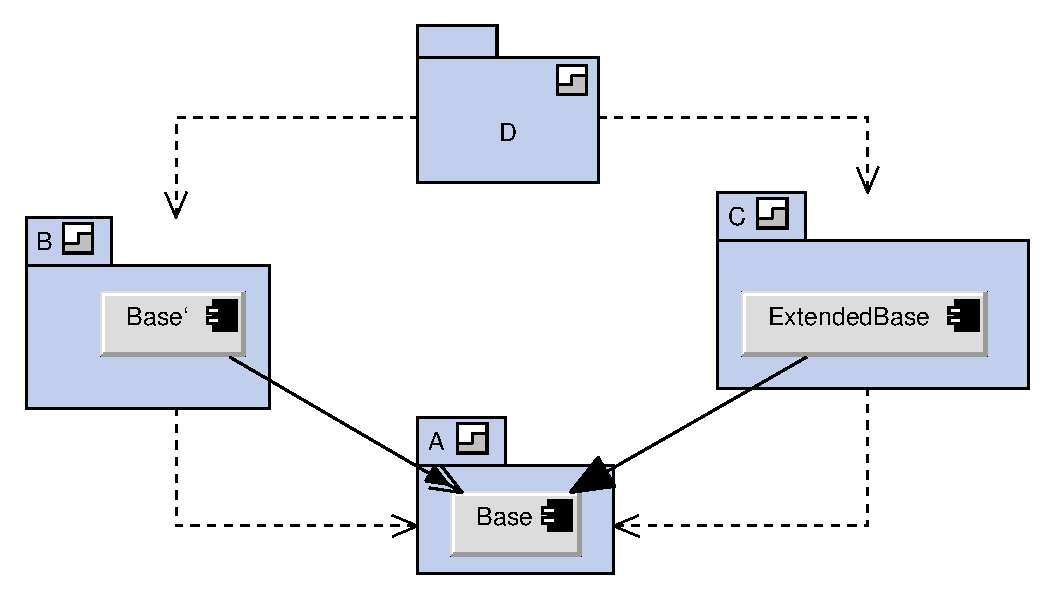
\includegraphics[width=1\columnwidth]{images/diamond}

\caption{\label{fig:A-diamond-dependency}A diamond dependency structure}



\end{figure}


The resemblance graph is reordered by taking substitution into account,
from the perspective of each stratum. This information is stored in
the resembles\_e field. For instance, from the perspective of C, NewBase
resembles Base. From the perspective of B, Base' also resembles Base.
From the perspective of D, however, NewBase resembles Base' which
then resembles Base. This reflects both the fact that Base' has been
substituted for Base and that Base' incrementally adjusts Base.

\begin{lyxcode}
{\scriptsize all~e:~Element~\{}{\scriptsize \par}

{\scriptsize{}~~all~s:~Stratum~\{}{\scriptsize \par}

{\scriptsize{}~~~~e.resembles\_e.s~=~}{\scriptsize \par}

{\scriptsize{}~~~~~~topmostOfSubstituted~+~topmostOfResemblance}{\scriptsize \par}

{\scriptsize{}~~~~...~\}}{\scriptsize \par}
\end{lyxcode}
In the above Alloy snippet, we set the resembles\_e relation for each
element to be the element it redefines (for incremental substitution
the rules are slightly different) \emph{or} the element it resembles,
taking into account the previous substitution rewriting from the depended
upon stratum. (In the model topmostOfSubstituted and topmostOfResemblance
are mutually exclusive)

Hence, the resembles\_e values for NewBase become ((Base, C), (Base',
D)). This rewriting of the resemblance graph, using the partial strata
dependency order, can result in multiple resemblance, however. Consider
if another substitution took place in stratum C (Base\_C'). From the
perspective of D, the resembles\_e values for NewBase would be ((Base\_C',
C), (Base\_C', D), (Base', D)). From this perspective, NewBase multiply
resembles both Base\_C' and Base'.

Once substitution has been factored into the resembles\_e relation,
the deltas are applied. In a purely linear resembles\_e graph, we
could just apply the deltas in order (add, delete, replace). Some
issues may occur still: for instance, NewBase may try to replace a
part which existed from the perspective of C, but is deleted by Base'
in the perspective of B and D. A small number of rules are defined
to deal with such situations and they are generally in accordance
with intuition.

With multiple resemblance, however, we may get legitimate conflicts.
For instance, Base' and Base\_C' may try to replace the same part.
In this case, both parts are present from the D perspective, and both
are associated with the same identifier. This flags up the Base component
(the component we are substituting) as being in error from this perspective.
A further incremental substitution (Base\_D') in D will result in
the following resembles\_e graph (figure X). As such, Base\_D is able
to make any corrections to handle the conflict. In this case, Base\_D'
can simply replace the part definitively with one of its own, or delete
it entirely either of which leaves Base error-free in D.

This type of conflict occurs when we try to combine independently
developed extensions into the same application. The conflicts cannot
be resolved automatically, as they represent different views of how
the underlying structure should look, at the same level of abstraction.
This type of conflict is to be expected in a model which offers such
flexibility to alter the base application, and it can be resolved
using the same constructs that led to the conflict: resemblance, substitution
and a further extension. 

Unique identifiers are vital to Backbone. Each component and constituent
(port, part etc) are allocated a universally unique identifier (UUID)
when first created (added). Subsequent replacement keeps the same
UUID, allowing replacement to work even in the presence of resemblance
graph re-ordering. UUIDs also allow the human readable names to change,
without affecting the identity of the elements. The UUIDs are managed
and kept hidden by the graphical CASE tool we have developed, and
the user only sees the names.


\section{\label{sec:Related-Work}Related Work}

Plugin architectures have been used successfully for many systems.
Eclipse is based on the OSGi module system, which provides full versioning
of plugins (bundles) and the export / import constructs \cite{O.Gruber2005}.
Firefox has plugins for handling media types \cite{Firefoxplugins2008}
along with more general additions \cite{Fireextensions2007}.

COM provides a compositional component model for Microsoft Windows
\cite{Box1997}. Microsoft Office applications are able to use this
as an extension approach, as scripts loaded into the applications
can call out to COM components \cite{Microsoft2006}. Component versions
are held in a global registry leading to a situation called {}``DLL
Hell'' when multiple applications require different versions of the
same component \cite{Stuckenholz2005}. The situation has improved
recently with {}``registration-free'' COM \cite{Templin2005}, which
allows applications to have their own local registry. However, this
does not address the problem of combining multiple extensions in a
single application.

A level of substitution can be achieved by COM registry adjustment,
but the inability to easily adjust conflicts upstream generally require
non-breaking changes to components only, ruling out some valid types
of extension. COM also embeds structure and occasionally object instantiation
in code, meaning that a uniform graphical treatment is difficult.

Interestingly, the term {}``plugin hell'' \cite{Birsan2005} has
also been coined which is not surprising since both the COM and plugin
approaches use a registry. 

Backbone is strongly influenced by architectural description languages,
including Darwin \cite{Magee1995}, UML2's composite structure model
\cite{Selic2003} and ROOM \cite{Selic1994}. Koala is an ADL which
is able to handle product line architectures through parametrization
and compile-time switches. Batory and others have long shown the practicality
of modeling a system via compositional components {[}ref].

Backbone can be used to handle component adaptation. The need for
adaptation and the integration problems of components are described
in \cite{Holzle1993}. Most approaches to this problem center around
component wrapping \cite{Bosch1999}.

The Backbone extension approach is closely related to the work done
in architectural configuration management (CM) \cite{Hoek2001,Roshandel2004}.
In a way, Backbone acts as a decentralized architectural CM system,
preventing the need to share a common repository. The approach also
prevents to incorporate extension points into a base architecture.

Product lines \cite{Eriksson2006}and populations \cite{Ommering2002}
provide a way to build up an application family from a set of related
requirements. The use of gluons and aspects in \cite{Batory2002}
provides many of the same features as our approach, but is not specifically
concerned with extensible applications.

Extensibility of systems is closely related to the notion of software
reuse. Object-oriented inheritance \cite{Taivalsaari1996} provides
the ability to make additive changes and for some (usually pre-planned)
replacement of methods only. Mixins are effectively abstract subclasses,
allowing functionality to be {}``mixed in'' to several classes \cite{Bracha1990}.
However, the use of mixins must be pre-planned, as they call into
methods of the superclass, and naming conflicts can occur when combining
multiple mixins into a single class.

UML2 contains the package merge construct, which allows packages to
be added together, effectively forming an additive union \cite{OMGUML}.
The specification of this presents several problems \cite{Zito2006},
and the fact that no replacement or deletion are allowed limits its
utility to extensible systems. Further, UML2 contains the notion of
redefinition. This is a form of inheritance on a component basis,
where the inheriting element can covariantly override the features
of the base. This is related to resemblance, but does not allow deletion
or arbitrary replacement.


\section{\label{sec:Conclusions-and-Future}Conclusions and Future Work}

Component substitution architectures offer a more flexible alternative
to plugin architectures, ameliorating or directly addressing the limitations
of the plugin model. The foundation of the approach is to allow an
extension to substitute any component in an application with one of
its own. Combined with resemblance, which allows components to structurally
inherit from each other, this allows an extension to incrementally
modify any part of the base application. Substitution and resemblance
in Backbone also apply to interfaces, providing a way to gracefully
evolve the service capabilities of components.

A key issue with the plugin model is the lack of a composition hierarchy.
Plugins cannot currently contain or nest other plugins -- they all
exist at the same level. Without the ability to nest, a fine-grained
model of the Eclipse architecture would involve many thousands of
plugins at the top level, and become extremely difficult to manage.
As a consequence, a plugin in Eclipse must be relatively coarse-grained.

A further problem is that the plugin model primarily facilitates additive
change. If modification of the existing plugins are required, because
the extension points are perhaps not present, then a new version will
have to be created. This characteristic of turning notional additive
change into replacement interacts badly with the coarse-grained nature
of the plugins, leading to great effort for simple changes. Further,
distributing a new version of a plugin can be impractical particularly
if others (including the primary source) are also releasing independently
updated versions.

Following on from this theme, the component substitution model contains
a fully hierarchical component model. A system modeled using composition
can be understood at the required abstraction level, and components
can be decomposed to be as fine-grained as desired, without creating
a complex and unworkable architecture.

The Backbone substitution and resemblance constructs, coupled with
the hierarchical component model, allow for fine-grained substitution
at the appropriate level of abstraction. The constructs form a simple,
but effective, decentralized version control system for a system architecture
and the keeping of changes as deltas allows multiple substitutions
to be combined.

Further, in Backbone every constituent of each component is a potential
extension point. This leads to systems which are extensible without
placing the burden on the application designer to try to predict and
factor in every possible extension point required. Compared to plugin
architectures, component substitution is shown to result in a simpler
system architecture, whilst also offering more power to extension
developers.

The component substitution approaches gives more flexibility, but
introduces an obvious issue compared to plugin architectures: we can
no longer guarantee that combining independently developed extensions
into a single application will not produce some structural conflicts.
To address this, we showed that a further extension can always be
used to rectify conflicts introduced in this way.

The current status of the work is as follows. The formal model has
been completed and used to implement a UML2-based case tool where
modeling with deltas is handled by always showing the full, expanded
structure of each component. This leads to a situation where component
extension is as straightforward as initial component modeling. The
previous interpreter is currently being rewritten to conform to the
formal model.

Future work will focus on expressing the behavioral properties of
components in an extension setting. We plan to express protocols using
sequence diagrams (with operators) which we will process into the
FSP process algebra \cite{Magee1999}. The individual protocols of
each part of a component will be composed to detect protocol violations
that occur when substituting components.

Other work includes a {}``baselining'' facility where progressive
deltas from extensions can be compressed into a new base system. This
will overcome the limitation of designing with an increasing set of
layered deltas.

\bibliographystyle{plain}
\bibliography{\string"../../read papers/references\string"}

\end{document}
